\section{Programming in the Cloud with GitHub}
\label{sec.github}


\begin{figure}[h]
  \centering
  \includegraphics[width=0.5\textwidth]{GitHub-How-to-use-GitHub-Edureka-300x241.png}
%%  \url{https://www.edureka.co/blog/how-to-use-github/}
  \caption{GitHub is a cloud service that hosts code repositories which 
    you can access via a web browser.}
\end{figure}

\subsection{Objectives}
The assignment in this section is:
\begin{enumerate}
\item Create a GitHub account
\item Open the \code{src/hello.py} with GitHub Code-Spaces.
\item Edit the code in two places.
\item Run the \emph{tests}  in \code{tests/test\_hello.py} using Code-Spaces
\end{enumerate}



\clearpage
\subsection{Create a GitHub Account}
\label{sec.account.create}
\begin{itemize}
\item \textbf{If you already have a GitHub account}: skip this section
(Section~\ref{sec.account.create}) and go directly to
Section~\ref{sec.github.login} (page \pageref{sec.github.login}).



\item \textbf{If you do not yet have a GitHub account}: you must create one.
Create a GitHub account using an abstract user name.  Don't use your
real name.  Instead use an artificial name use as your name from
Instagram or other social media.  You may also make up a completely
new name as long as no other person has already used that name on
GitHub.  \url{https://github.com/join}.  To complete the process of
creating a GitHub account you may need to authenticate using your
mobile phone.


\noindent\includegraphics[width=0.55\textwidth]{github-join.png}

\end{itemize}

\subsection{Log In to GitHub}
\label{sec.github.login}

If you are not already logged into GitHub, you should login at \url{https://github.com}.

\noindent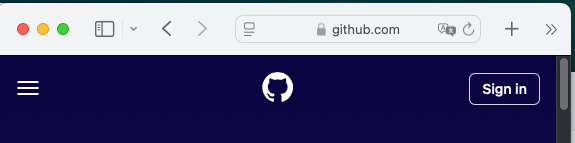
\includegraphics[width=0.8\textwidth]{github-signin.png}


\clearpage
\subsection{Open the Repository}
\label{sec.open.repo}
  


Open \url{https://github.com/jimka2001/immersion} with your web browser.  This makes the project visible to you.

\nopagebreak
\noindent\includegraphics[width=0.7\textwidth]{github-immersion.png}


\subsection{Fork yourself a copy}

Fork the repository.  This gives you a private copy.  You will make changes
necessary changes in the code using this private copy.

\nopagebreak
\noindent \includegraphics[width=0.6\textwidth]{github-fork-repo.png}



\subsection{Open a Python File in Code-Spaces}
  
\begin{enumerate}
\item Navigate to \code{src/hello.py} in the GitHub file browser, to see something like this.
  
\nopagebreak
\noindent\includegraphics[width=0.9\textwidth]{find-hello.png}



\item Click \code{hello.py} to open the file in an editor pane.  You
  should see something like what is shown here:
  
\nopagebreak
\noindent\includegraphics[width=0.9\textwidth]{hello-function.png}


\item Open the file by clicking \code{github.dev} not \code{Edit in place}.
  
\nopagebreak
\noindent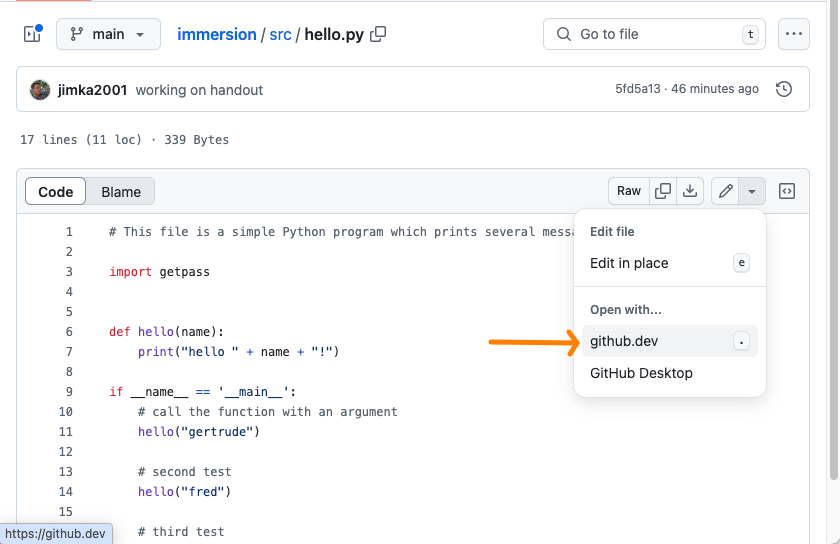
\includegraphics[width=0.85\textwidth]{github-dev.png}


\item You may need to wait while setting up. If this setup seems to
  never finish, it may mean you need to use Chrome as your web
  browser.
  
\nopagebreak
\noindent\includegraphics[width=0.3\textwidth]{github-dev-setup.png}


\item GitHub may ask for permission to see your repository.  Click on \textbf{Allow}.
  
  \nopagebreak
\noindent\includegraphics[width=0.65\textwidth]{github-ask-permission.png}
  

\item GitHub may ask for your GitHub ID.  Normally you just select the default one.
  
  \nopagebreak
\noindent\includegraphics[width=0.66\textwidth]{github-ask-user-name.png}

\item Finally, the GitHub development environment should be opened.
  
  \nopagebreak
\noindent\includegraphics[width=0.6\textwidth]{github-dev-opened.png}



\end{enumerate}

\subsection{Set up the Editor}
  
\begin{enumerate}

\item Now you can edit your code but you cannot run nor test it.

\item Find the icon \includegraphics[width=2cm]{run-debug.png} on the
  left hand side of the browser window.  Press that icon to see the
  following message.

\nopagebreak
\noindent\includegraphics[width=0.6\textwidth]{continue.png}

\item Press continue, and you should see a prompt such as the
  following to create a code space.

\nopagebreak
\noindent\includegraphics[width=0.9\textwidth]{create-code-space.png}

\item Select \includegraphics[width=8cm]{select-create.png}.

\item You may be asked how many cores do you want.

\nopagebreak
\noindent\includegraphics[width=0.9\textwidth]{select-cores.png}

\item You should select the minimum: \includegraphics[width=7cm]{two-cores.png}.

\item You'll probably now need to reopen the \code{src/hello.py} file.

\nopagebreak
\noindent\includegraphics[width=0.9\textwidth]{re-open-python-file.png}

\item You may be asked to install the Python extension.  Press \textbf{Install}.

\nopagebreak
\noindent\includegraphics[width=0.8\textwidth]{install-python-extension.png}

  

\item After it finishes installing,   you should see something like this:

\nopagebreak
\noindent\includegraphics[width=0.9\textwidth]{python-extension.png}

\item Reopen the explorer: \includegraphics[width=7cm]{explorer2.png},
  and select the \code{src/hello.py} file.

\nopagebreak
\noindent\includegraphics[width=0.4\textwidth]{explorer.png}
\end{enumerate}

\clearpage


% LocalWords:  GitHub atelier IDE CodeSpaces github
